This part of the thesis focuses on the equivalence between \wlnn and \gnn. We will begin by providing a preliminary section that formalizes all the concepts used in the proof and introduces a general notation. Afterward, we will dedicate a separate section to present and prove two theorems. These theorems combined conclude the equivalence proof.

\section{Preliminaries}\label{sec:pre_lim}
This section will introduce and formalizes all concepts used throughout the proof and the rest of the thesis. We start with general notations, introduce a general graph definition, and familiarize the reader with the Weisfeiler-Leman algorithm. We will introduce each framework independently, first the \wlnn and then \gnn. In the end, we will briefly introduce important properties of collections of functions computed by both methods.

\subsection{General Notation}
Let $\Nb$ denote the set of natural numbers such that $\Nb := \{0, 1,2, \ldots \}$. By $[n]$, we denote the set $\{0, \ldots, n\} \subset \mathbb{N}$ for each $n \in \mathbb{N}$. Further, with $\MSopen \ldots \MSclose$, we denote a multiset formally defined as a 2-tuple $(X, m)$, where $X$ is a set of all unique elements and $m: X \rightarrow \mathbb{N}_{\geq 1}$ a mapping that maps each element in $X$ to the number of its occurrences in the multiset.\todo{Changed $[n]$ to contain $0$}

\subsection{Graphs}
We will briefly introduce a formal definition for graphs and coloring on graphs. Starting with the definition of a graph.

\begin{definition}[Graph]
A graph $G$ is defined as a 3-tuple denoted by $G \coloneqq (V, E, l)$. This tuple consists of a set of nodes $V \subset \Nb$, a set of edges $E \subseteq V \times V$, and a labeling function $l: M \rightarrow \Sigma$. The domain $M$ of the labeling function can be either $V$, $V \cup E$, or $E$, and the codomain $\Sigma$ is a finite alphabet with $\Sigma \subset \mathbb{N}^k$, where $k \in \Nb$ is arbitrary.
In the context of this thesis, the assigned values by the labeling function are referred to as either labels or features, depending on the dimension of $\Sigma$. In detail, if $k=1$, we usually refer to the values as labels, otherwise as features. Additionally, the set of all graphs is denoted by $\cG$.

Furthermore, a graph $G$ can be either directed or undirected based on the definition of its set of edges $E$. If $E \subseteq \{(v,u) \mid v,u \in V\}$, it represents a directed graph, whereas if $E \subseteq \{(v, u) \mid v,u \in V, v\neq u\}$ such that for every $(v,u) \in E$ there exists $(u,v) \in E$, it defines an undirected graph. Additionally, for ease of notation, we will use $V(G)$ and $E(G)$ to denote the set of nodes and the set of edges of $G$, respectively, as well as $l_G$ to denote the label function of $G$. Further, with $\mathcal{N}(v)$ for $v \in V(G)$ we denote the set of neighbors of $v$ defined as $\mathcal{N}(v) \coloneqq \{u \mid (u, v) \in E(G)\}$, and with $d(v)$ for $v \in V(G)$ the degree of node $v$, defined as $d(v) := |\mathcal{N}(v)|$.
\end{definition}

We continue with the definition of a graph coloring.

\begin{definition}[Graph Coloring]
A coloring of a Graph $G$ is a function $C: V(G) \rightarrow \mathbb{N}$ that assigns each node in the graph a color (here, a positive integer). Further, a coloring $C$ induces a partition $\cP$ on the set of nodes, for which we define $C^{-1}$ being the function that maps each color $c \in \mathbb{N}$ to its class of nodes with $C^{-1}(c) = \{ v\in V(G) \mid C(v) = c\}$. In addition, we define $h_{G, C}$ as the histogram of graph $G$ with coloring $C$ that maps every color in the image of $C$ under $V(G)$ to the number of occurrences. In detail, $\forall c \in \mathbb{N}: h_{G, C}(c) \coloneqq | \{ v \in V(G) \mid C(v) = c \} | = | C^{-1}(c) |$.
\end{definition}

\subsubsection{Permutation-invariance and -equivariance}
We use $S_n$ to denote the symmetric group over the elements $[n]$ for any $n \in \Nb$. $S_n$ consists of all permutations over these elements. Let $G$ be a graph with $V(G) = [n]$, applying a permutation $\pi \in S_n$ on $G$, is defined as $G_\pi \coloneqq \pi \cdot G$ where $V(G_\pi) = \{\pi(0), \ldots, \pi(n) \}$ and $E(G_\pi) = \{ (\pi(v), \pi(u)) \mid (v,u) \in E(G)\}$. We will now introduce two key concepts for classifying functions on graphs.

\begin{definition}[Permutation Invariant]
    Let $f: \mathcal{G} \rightarrow \mathcal{X}$ be an arbitrary function, then $f$ is \textit{permutation-invariant} if and only if for all $G \in \mathcal{G}$, where $n_G \coloneqq \mid V(G) \mid$ and for every $\pi \in S_{n_G}$: $f(G) = f(\pi \cdot G)$.
\end{definition}

\begin{definition}[Permuation Equivariant]
    Let $f: \mathcal{G} \rightarrow \mathcal{X}$ be an arbitrary function, then $f$ is \textit{permuation-equivariant} if and only if for all $G \in \mathcal{G}$, where $n_G \coloneqq \mid V(G) \mid$ and for every $\pi \in S_{n_G}$: $f(G) = \pi^{-1} \cdot f(\pi \cdot G)$.
\end{definition}

\subsection{Weisfeiler and Leman Algorithm}\label{sec:1-WL Definition}
The Weisfeiler-Leman algorithm consists of two main parts, first the coloring algorithm and second the graph isomorphism test. We will introduce each part individually.

\subsubsection{The Weisfeiler-Leman Graph Coloring Algorithm}
The $\wl$ algorithm computes a node coloring of its input graph in each iteration. In detail, a color is assigned to each node based on the colors of its neighbors and its own current color. The algorithm continues until convergence is reached, resulting in the final coloring of the graph. We will now formally define this procedure and provide an illustrative example in \cref{fig:1wl_example}.

\begin{definition}[$\wl$ Algorithm]
    Let $G = (V, E, l)$ be a labeled graph. In each iteration $i$, the \wl algorithm computes a node coloring $C_i: V(G) \rightarrow \mathbb{N}$. In the initial iteration $i=0$, the coloring is set to $C_0 = l$ if $l$ exists. Otherwise, for all $v \in V(G): C_0(v) = c$ with $c \in \Nb$ being an arbitrary but fixed constant. For $i > 0$, the algorithm assigns a color to $v \in V(G)$ as follows:
    \begin{equation*}
        C_i (v) = \textsf{RELABEL}(C_{i-1}(v),  \ \MSopen C_{i-1}(u) \mid u \in \mathcal{N}(v) \MSclose),
    \end{equation*}
    where $\textsf{RELABEL}$ injectively maps the above pair to a unique, previously not used, color. The algorithm terminates when the number of colors between two iterations does not change, meaning the algorithm terminates after iteration $i$ if the following condition is satisfied:
    \begin{equation*}
        \forall v,w \in V(G):  C_i(v) = C_i(w) \iff C_{i+1}(v) = C_{i+1}(w).
    \end{equation*}
    Upon terminating we define $C_{\infty} \coloneqq C_i$ as the stable coloring, such that $\wl(G) \coloneqq C_\infty$.
\end{definition}

The colorings computed in each iteration always converge to the final one, such that the algorithm always terminates. In more detail, \cite{Gro2017} showed that it always holds after at most $|V(G)|$ iterations. For an illustration of this algorithm, see \autoref{fig:1wl_example}. Moreover, based on the work of \cite{Pai+87} about efficient refinement strategies, \cite{Car+82} proved that the stable coloring $C_\infty$ can be computed in time $\mathcal{O}(| V(G) | + |E(G)| \cdot \log | V(G) |)$.

\begin{figure}[H]
    \centering
    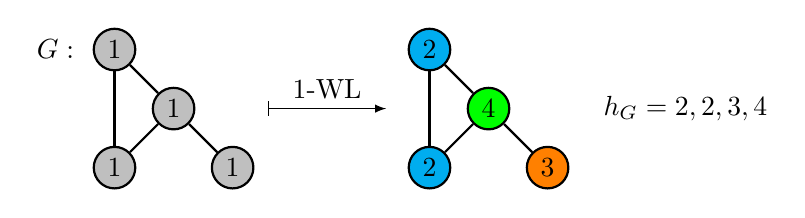
\begin{tikzpicture}
    \tikzset{line/.style={draw,thick}}
    \tikzset{arrow/.style={line,->,>=stealth}}
    \tikzset{node/.style={circle,inner sep=0pt,minimum width=15pt}}
    
    \draw (-1.5,0.75) node {$G:$};
    \node[line,node,fill=lightgray] (x1) at (-0.75, 0.75) {1};
    \node[line,node,fill=lightgray] (x2) at (-0.75, -0.75) {1};
    \node[line,node,fill=lightgray] (x3) at (0.75, -0.75) {1};
    \node[line,node,fill=lightgray] (x4) at (0, 0) {1};
    
    \path[line] (x1) to (x2);
    \path[line] (x1) to (x4);
    \path[line] (x2) to (x4);
    \path[line] (x3) to (x4);

    \draw [|-latex] (1.2,0) -- node [text width=2.5cm,midway,above,align=center ] {1-WL} (2.7,0);
    

    \node[line,node,fill=cyan] (x1) at (-0.75 + 4.0, 0.75) {2};
    \node[line,node,fill=cyan] (x2) at (-0.75 + 4.0, -0.75) {2};
    \node[line,node,fill=orange] (x3) at (0.75 + 4.0, -0.75) {3};
    \node[line,node,fill=green] (x4) at (0 + 4.0, 0) {4};
    
    \path[line] (x1) to (x2);
    \path[line] (x1) to (x4);
    \path[line] (x2) to (x4);
    \path[line] (x3) to (x4);

    \draw (6.5, 0.0) node {$h_G = \MSopen 2, 2, 3, 4 \MSclose$};

    
    
    \end{tikzpicture}

    \caption{An example of the final coloring computed by applying the \wl algorithm on the graph $G$. The graph $G$ consists of $4$ nodes with all their labels being set to the same color.}
    \label{fig:1wl_example}
\end{figure}

It is important to understand that since the algorithm was originally developed as a simple heuristic for the \textit{graph isomorphism problem}, which is an inherently discrete problem, the \wl algorithm in its simplest form, as we presented it here, does only work on graphs with discrete, one-dimensional node labels. Although it is quite easy to adapt the algorithm to respect discrete edge labels of a graph by using them as weights in the neighborhood aggregation (\cite{Shervashidze2011}), modifying its definition to work with continuous graph features is more complex. Numerous proposed modifications have been put forward to address this integration in the literature, such as those discussed by \cite{Mor+2016}. However, note that this particular topic will not be further investigated in this thesis, although its mention holds value for \cref{sec:discussion}, in which we will discuss the insights we obtained for \gnns.

\subsubsection{The Weisfeiler-Leman Graph Isomorphism Test}
The isomorphism test uses the \wl coloring algorithm and is defined as follows.

\begin{definition}[$\wl$ Isomorphism Test]
    To determine if two graphs $G, H \in \mathcal{G}$ are non-isomorphic ($G \ncong H)$, one applies the \wl coloring algorithm on both graphs ``in parallel'' and checks after each iteration if the occurrences of each color are equal, else the algorithm would terminate and conclude non-isomorphic. Formally, the algorithm concludes non-isomorphic in iteration $i$ if there exists a color $c$ such that: 
    \begin{equation*}
        |\{ v \in V(G) \mid C_i(v) = c\} | \neq |\{ v \in V(H) \mid C_i(v) = c\} |.
    \end{equation*}
\end{definition}

Note that this test is only sound and not complete for the \textit{graph isomorphism problem}. Counterexamples can be easily constructed where the algorithm fails to distinguish non-isomorphic graphs. See \autoref{1-WL Counter Example} for a straightforward example of where this test fails that was discovered and proven by \cite{Cai1992}.
\begin{figure}[H]
    \centering
    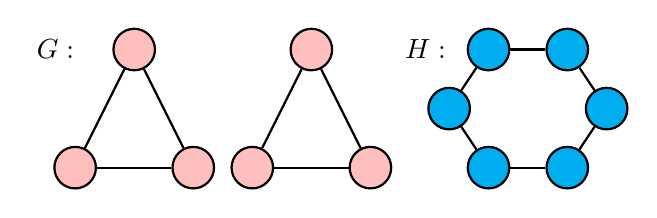
\begin{tikzpicture}

\tikzset{line/.style={draw,thick}}
\tikzset{arrow/.style={line,->,>=stealth}}
\tikzset{node/.style={circle,inner sep=0pt,minimum width=15pt}}

\draw (-1.0,0.75) node {$G:$};
\node[line,node,fill=pink] (x1) at (0, 0.75) {};
\node[line,node,fill=pink] (x2) at (-0.75, -0.75) {};
\node[line,node,fill=pink] (x3) at (0.75, -0.75) {};

\path[line] (x1) to (x2);
\path[line] (x1) to (x3);
\path[line] (x2) to (x3);

\node[line,node,fill=pink] (x1) at (2.25, 0.75) {};
\node[line,node,fill=pink] (x2) at (1.5, -0.75) {};
\node[line,node,fill=pink] (x3) at (3.0, -0.75) {};

\path[line] (x1) to (x2);
\path[line] (x1) to (x3);
\path[line] (x2) to (x3);

\draw (3.7, 0.75) node {$H:$};
\node[line,node,fill=cyan] (x1) at (3.75 + 0.25, 0) {};
\node[line,node,fill=cyan] (x2) at (4.25 + 0.25, 0.75) {};
\node[line,node,fill=cyan] (x3) at (5.25 + 0.25, 0.75) {};
\node[line,node,fill=cyan] (x4) at (5.75 + 0.25, 0) {};
\node[line,node,fill=cyan] (x5) at (5.25 + 0.25, -0.75) {};
\node[line,node,fill=cyan] (x6) at (4.25 + 0.25, -0.75) {};

\path[line] (x1) to (x2);
\path[line] (x2) to (x3);
\path[line] (x3) to (x4);
\path[line] (x4) to (x5);
\path[line] (x5) to (x6);
\path[line] (x6) to (x1);

\end{tikzpicture}
    \caption{This is an example of two graphs $G$ and $H$ that are non-isomorphic but cannot be distinguished by the \wl isomorphism test.}
    \label{1-WL Counter Example}
\end{figure}

\subsubsection{Implications of the \wl Algorithm}
One intriguing implication of the \wl algorithm and its isomorphism test is that, due to it not being complete for solving the \textit{graph isomorphism problem}, it gives rise to a related but weaker relation than the isomorphism relation ($\simeq$). We define this relation as follows.

\begin{definition}[\wl Relation]
    Let $\cX \subseteq \cG$. For any graphs $G,H \in \cX$ we will denote $G \wliso H$ if the \wl isomorphism test can not distinguish both graphs. Note that due to the soundness of this algorithm, if $G \not\wliso H$, we always can conclude that $G \not\simeq H$.
\end{definition}

The $\wliso$ relation can further be classified as an equivalence relation, as it is reflexive, symmetric and transitive. With this, we introduce a notation of its equivalence classes. Let $\cX \subseteq \cG$ and $G \in \cX$, then we denote with $\cX/\!{\wliso}(G): = \{ G' \in \cX \mid G \wliso G' \}$ its equivalence class.

Similarly, we define the notion \wldisc for collections of permutation invariant functions. 

\begin{definition}[\wldisc]
    Let $\cX \subseteq \cG$. Further, let $\mathcal{C}$ be a collection of permutation invariant functions from $\cX$ to $\Rb$. We say $\mathcal{C}$ is \textbf{\wldisc} if for all graphs $G_1, G_2 \in \mathcal{X}$ for which the \wl isomorphism test concludes non-isomorphic ($G_1 \not\wliso G_2$), there exists a function $h \in \mathcal{C}$ such that $h(G_1) \neq h(G_2)$.
\end{definition}

\subsection{$\wlnn$}\label{sec:definition_wlnn}
As the previous section shows, the $\wl$ algorithm is quite powerful in identifying a graph's substructures and distinguishing non-isomorphic graph pairs. With the $\wlnn$ framework, we define functions that utilize this structural information to derive further application-specific insights.

\begin{definition}[$\wlnn$]
    A $\wlnn$ model consists of three components that are applied sequentially to its input: 1. the $\wl$ algorithm, 2. an encoding function $f_\text{enc}$ operating on graph colorings, and 3. an arbitrary multilayer perceptron $\mlp$. In detail, a \wlnn model computes the function $\cB$, that is defined as follows:
    \begin{align*}
        \cB: \cG \rightarrow \Rb^k, \ G \mapsto \text{MLP} \circ f_{\text{enc}}(\MSopen \wl(G)(v) \mid v \in V(G) \MSclose),
    \end{align*}
    where ``$\wl(G)$'' is the coloring computed by the $\wl$ algorithm when applied on $G$, and $k \in \Nb$ is an arbitrary constant. For a better understanding and an illustrative explanation, see \cref{fig:wlnn}.
\end{definition}

It is worth noting that this definition can be easily adjusted to accommodate node or edge-related tasks by applying the encoding function $f_\text{enc}$ and the multilayer perceptron $\mlp$ elementwise to the colors of the multiset. However, for the purposes of this thesis, we will not delve into these variations, as our main focus will be on graph-wide tasks such as graph classification or regression, which possess greater theoretical interest and are more prevalent in most datasets. Furthermore, all the theoretical findings presented in this thesis can also be applied to $\wlnn$ models designed for node or edge tasks.

\begin{figure}[!htb]
    \centering
    \begin{tikzpicture}
    \definecolor{pastell_blue}{RGB}{133,154,202}
    \definecolor{pastell_green}{RGB}{192,223,211}
    \definecolor{pastell_pink}{RGB}{228,197,212}
    \tikzset{line/.style={draw,thick}}
    \tikzset{arrow/.style={line,->,>=stealth}}
    \tikzset{node/.style={circle,inner sep=0pt,minimum width=15pt}}
    
    \node[line,node,fill=gray] (x1) at (-0.75 - 0.8, 0.75) {};
    \node[line,node,fill=gray] (x2) at (-0.75 - 0.8, -0.75) {};
    \node[line,node,fill=gray] (x3) at (0.75 - 0.8, -0.75) {};
    \node[line,node,fill=gray] (x4) at (0 - 0.8, 0) {};
    
    \path[line] (x1) to (x2);
    \path[line] (x1) to (x4);
    \path[line] (x2) to (x4);
    \path[line] (x3) to (x4);

    \draw[arrow, thick] (0.1, 0.0) to (0.9, 0.0);

    \draw (2.15, 0.9) node {$\wlnn$:};
    \filldraw[draw=black, fill=gray!40, thick, rounded corners] (1.1, -0.7) rectangle (8.9, 0.7);

    \filldraw[draw=black, fill=green, thick, rounded corners] (1.2, -0.6) rectangle (2.4, 0.6) node[midway,align=center]{$\wl$};

    \draw[arrow, thick] (2.5, 0.0) to (2.9, 0.0);
    
    \draw (3.5, 0.0) node {$\MSopen \ldots \MSclose$};

    \draw[arrow, thick] (4.1, 0.0) to (4.5, 0.0);

    \filldraw[draw=black, fill=cyan, thick, rounded corners] (4.6, -0.6) rectangle (5.8, 0.6) node[midway,align=center]{$f_{\text{enc}}$};

    \draw[arrow, thick] (5.9, 0.0) to (6.3, 0.0);
    \draw (6.7, 0.0) node {$\begin{pmatrix*} \vdots \end{pmatrix*}$};
    \draw[arrow, thick] (7.1, 0.0) to (7.5, 0.0);

    \filldraw[draw=black, fill=pink, thick, rounded corners] (7.6, -0.6) rectangle (8.8, 0.6) node[midway,align=center]{$\mlp$};

    \draw[arrow, thick] (9.1, 0.0) to (9.9, 0.0);
    \draw (10.3, 0.0) node {$42$};
    
\end{tikzpicture}

    \caption{This simplified illustration explains the components that make up a \wlnn model and how each one processes the input further. In detail, the model takes the graph on the left as input and first applies the \wl algorithm, thereby obtaining a multiset of the colors assigned by the algorithm. Then the encoding function $f_\text{enc}$ is applied, resulting in a fixed-sized vector that is further processed by the multilayer perceptron $\mlp$. The output of the $\mlp$ is then propagated as the $\wlnn$ models output, here the number $42$.}
    \label{fig:wlnn}
\end{figure}

\subsection{Graph Neural Networks (Message-Passing)}\label{sec:GNN Defintion}
A \textsf{Graph Neural Network} (\gnn) is a composition of multiple layers, where each layer computes a new feature for each node and edge. Each \gnn layer thus technically obtains a new graph structurally identical to the previous one but contains new feature information. After an input graph has been passed through all layers, a final readout function is applied that pools all graph features and derives a task-related output. With this, it is possible to apply a \gnn to every graph, regardless of its size, as the ``computation'' will only take place on the nodes and edges of the graph.

Note that in the following, we will restrict the definition only to consider node features; however, one can easily extend it to include edge features as well.

\begin{definition}[\textsf{Graph Neural Network}]\label{def:gnn}
    Let $G = (V, E, l)$ be an arbitrary graph. A \textsf{Graph Neural Network} (\gnn) is a composition of multiple layers and a final readout function where each layer $t$ is represented by a function $f^{(t)}$. The initial layer at $t=0$ is a functioning of the format $f^{(0)}: V(G) \rightarrow \mathbb{R}^{1 \times d}$ that is consistent with $l$ and translates all labels into a vector representation. In contrast, for every $t > 0$, $f^{(t)}$ is recursively defined as:
    \begin{align*}
        f^{(t)}(v) = f^{(t)}_{\text{merge}} (f^{(t-1)}(v), \  f^{(t)}_{\text{agg}}( \MSopen f^{(t-1)}(w) \mid w \in \mathcal{N}(v) \MSclose )),
    \end{align*}
    where $f^{(t)}_{\text{merge}}$ is an arbitrary function that maps the aforementioned tuple to a vector, effectively ``merging'' them, while $f^{(t)}_{\text{agg}}$ is an arbitrary function that maps the multiset to a vector, effectively ``aggregating'' it.
    
    The readout function, referred to as $\textsf{Readout}$, is applied after the input graph has been passed subsequently through all layers and is defined as follows:
    \begin{align*}
        \textsf{Readout}(\MSopen f^{(t)}(v) \mid v \in V(G) \MSclose).
    \end{align*}
    This function pools the information from every node feature, processes it, and calculates a fixed-sized output vector for the entire graph.
    
    In summary, a \gnn model will compute the function $\cA$ defined as follows:
    \begin{align*}
        \mathcal{A}: \cG \rightarrow \Rb^k, \ G \mapsto \textsf{Readout}(\MSopen f^{(T)}(v) \mid v \in V(G) \MSclose),
    \end{align*}
    where $T$ is the number of layer of the \gnn, and $k \in \Nb$ an arbitrary constant. To enable end-to-end training of a \gnn, it is essential that all its components are differentiable. Therefore, we require all $f^{(t)}_{\text{merge}}$ and $f^{(t)}_{\text{agg}}$ functions for all $t \in [T]$, along with the final $\textsf{Readout}$ function, to be differentiable.
\end{definition}
Note that, due to our definition of the ``aggregation'' and the ``readout'' function to operate over multisets, both functions are permutation invariant by definition. With this, we can conclude that the total composition $\mathcal{A}$ is permutation invariant, and with similar reasoning, it is also differentiable. This property enables us to train $\mathcal{A}$ like any other machine learning method in an end-to-end fashion, regardless of the underlying encoding used for graphs. Furthermore, \gnns following this definition are regarded as \textsf{Message-Passing-Neural-Network (MPNN)}. This designation stems from each node exchanging information with its direct neighbors in each layer. As a result, information during the processing of a graph is propagated by passing many messages across the graph; thus, these layers are also referred to as message-passing layers. As outlined in the introduction to this thesis, we will solely focus on \gnns utilizing the message-passing architecture. Therefore we will use the term \gnn and \textsf{MPNN} interchangeably throughout this thesis. The definition and notation used here are inspired by \cite{Morris2018} and \cite{Xu2018}.

To bridge the gap from the theoretical definition to practical instances of the definition, we will now introduce three distinct \gnn architectures. Specifically, we will explore the \textsf{Graph Attention Network (GAT)} developed by \cite{Velivckovic2017}, \textsf{Graph Convolutional Network (GCN)} proposed by \cite{Kip+2017}, and the \textsf{Graph Isomorphism Network (GIN)} introduced by \cite{Xu2018}. These architectures will serve as empirical baselines in \cref{part2}. Additionally, we will also elaborate on the reasons for this choice of models in \cref{part2} in \cref{sec:gnn_model_choice}. We listed the definitions of the message-passing layers of each model in \cref{tab:models}.

\begin{table}[!htb]
    \centering
    \caption{Overview of the construction of the message-passing layers and their respective learnable parameters by popular \gnn model. This format is inspired by \cite{Nikolentzos2023}.}
    \label{tab:models}
    \resizebox{.975\textwidth}{!}{ 	\renewcommand{\arraystretch}{1.05}
    \begin{tabular}{ c| c |c}
        \textbf{Model} & \textbf{Message-Passing Layer Definition} & \textbf{Learnable Parameters}\\
        \hline
        GCN & $f^{(t)}(v) = \text{ReLU}\biggl( \sum_{u \in \cN(v) \cup \{v\}} \frac{W^{(t)}}{\sqrt{(1 + d(v))(1 + d(u))}} f^{(t-1)}(u)\biggr)$ & $W^{(t)}$ \\
        \hline
        GIN & $f^{(t)}(v) = \mlp^{(k)} \biggl( (1 + \epsilon^{(k)}) f^{(t-1)}(v) + \sum_{u \in \cN(v)} f^{(t-1)}(u)\biggr)$ & $\epsilon^{(k)}, \mlp^{(k)}$\\
        \hline
        GAT & $f^{(t)}(v) = \sigma \biggl( \sum_{u \in \cN(v)} \alpha_{vu} W^{(t)} f^{(t-1)}(u) \biggr)$ & $\alpha_{vu}, W^{(t)}$\
    \end{tabular}}
\end{table}

Commonly employed \textsf{Readout} functions in this context often involve straightforward pooling techniques like elementwise summation, mean calculation, or maximum extraction. These pooling operations are typically followed by a multilayer perceptron, which performs additional processing on the aggregated information. Although more sophisticated pooling operations exist, such as \textsc{Set2Set} developed by \cite{Vinyals2015}, \cite{Xu2018} showed that given the correct configuration, the elementwise summation pooling function combined with a following multilayer perceptron suffices to create a \gnn that is as expressive as the \wl algorithm in distinguishing non-isomorphism.

\section{Theoretical Connection}\label{sec:theo_connections}
This section is the main part of our theoretical investigation of the two frameworks \wlnn and \gnn. We will present three intriguing theorems, which will be proven separately afterward. In detail, the first two theorems will establish an equivalence between the two frameworks when the input set of graphs is finite. While the last theorem will take this a step further and demonstrate how powerful the \wl algorithm is, establishing a connection for continuous functions computed by \wlnn and \gnn proves a somewhat weaker connection between them.

In the first two theorems, we focus on a finite collection of graphs, which we denote by $\cX$ with $\cX \subset \cG$.
\begin{theorem}[Finite Case: ``$\text{GNN} \subseteq \wlnn$'']\label{theorem:1wl_in_gnn}
    Let $\cC$ be a collection of functions from $\cX$ to $\Rb$ computable by \gnns, then $\cC$ is also computable by $\wlnn$.
\end{theorem}

\begin{theorem}[Finite Case: ``$\wlnn \subseteq \text{GNN}$'']\label{theorem:gnn_in_1wl}
    Let $\cC$ be a collection of functions from $\cX$ to $\Rb$ computable by $\wlnn$, then $\cC$ is also computable by \gnns.
\end{theorem}
With these two theorems, the equivalence between both frameworks follows. Specifically, every function computed by \wlnn working over any arbitrary, but finite $\cX \subset \cG$ is also computable by a \gnn, and vice versa. As we move towards the empirical evaluation in \cref{part2}, it is evident that if we test a \wlnn model on any of the benchmark datasets, it can achieve the same level of performance as a \gnn model. Notice that we did not leverage any constraints on the encoding of graphs throughout the first two theorems and their corresponding proves but instead kept it general.

Having established a connection between the two frameworks on a finite subset of graphs, we wanted to further demonstrate the expressive power of the \wl algorithm and in particular of collections of functions that are \wldisc by investigating a connection between the two frameworks for continuous feature spaces and continuous functions. However, since the \textit{graph isomorphism problem} is an inherently discrete problem, the \wl algorithm, as outlined in \cref{sec:definition_wlnn}, is only defined as a discrete and discontinuous function operating on discrete colors, such that extending the definition of the \wl algorithm to a continuous function working over continuous values is not very trivial and, to our knowledge, has not yet been widely investigated. Therefore, we assume in the proof and the following theorem that a continuous version of the \wl algorithm exists. \todo{Continous version of wl wo genannt wieder abändern}

We define the set of graphs with continuous labels using the following definition:
\begin{definition}
    Let $X$ be a compact subset of $\Rb$ including $0$. We decode graphs with $n$ nodes as a matrix $G \in X^{n \times n}$, where $G_{i,i}$ decodes the label of node $i$ for $i \in [n]$, and $G_{i,j}$ with $i \neq j \in [n]$ decodes an edge from node $i$ to $j$ and a corresponding edge features. Furthermore, we say that there is an edge between node $i$ and $j$ if and only if $G_{i,j} \neq 0$. Additionally, if $G$ encodes an undirected graph, $G$ is a symmetric matrix. For simplicity, we denote $\cX \coloneqq X^{n \times n}$ throughout the next two theorems and their respective proofs.
\end{definition}

\begin{theorem}[Continuous Case: ``$\text{GNN} \subseteq \wlnn$'']\label{theorem:1wl_in_gnn_approximating}
    Let $\cC$ be a collection of continuous functions from $\cX$ to $\Rb$ computable by $\wlnn$. If $\cC$ is \wldisc, then there exists a collection of functions $\cC'$ computable by $\wlnn$ that is \gnn-Approximating.
\end{theorem}

Since we only wanted to show the expressive power of \wldisc and made the major assumption of the existence of a continuous $\wl$ algorithm, we have included the proofs of \cref{theorem:1wl_in_gnn_approximating,theorem:gnn_approximating_in_1wl} in the Appendix in \autoref{app:gnn_in_wlnn}.

By putting both theorems into perspective, we can now argue that even for continuous functions $\wlnn$ and \gnns can compute almost the same functions. Each framework can approximate the other framework arbitrarily well. We can conclude that the ability \wldisc is very powerful, so we can assume that $\wlnn$ is sufficiently expressive for the upcoming empirical part.

\subsection{Proof of \autoref{theorem:1wl_in_gnn}}\label{sec:proof_theorem:1wl_in_gnn}
We will prove \autoref{theorem:1wl_in_gnn} by introducing a couple of small lemmas, which combined prove the theorem. In detail, in \autoref{lem:wl_disc_exists}, we show the existence of a collection computed by $\wlnn$ that is 1-\!WL-Discriminating. In \cref{lem:wlnn_permutation_invariance,lem:wl_relation_equivalence,lem:composition_lemma} we derive properties of $\wlnn$ functions we will use throughout \cref{lem:encoding-indicator-func1,lem:encoding-indicator-func2,lem:decompose_gnn_as_wl} with which we prove the theorem.
We took great inspiration for \cref{lem:encoding-indicator-func1,lem:encoding-indicator-func2,lem:decompose_gnn_as_wl} from the proof presented in section 3.1 in the work of \cite{Chen2019}.

\begin{lemma}\label{lem:wl_disc_exists}
    There exists a collection $\cC$ of functions from $\cX$ to $\Rb$ computable by $\wlnn$ that is 1-\!WL-Discriminating.
\end{lemma}

\begin{proof}
    We define $f_c$ for $c \in \Nb$ as the encoding function that returns the number of nodes colored as $c$. With this, we can construct the collection of functions $C$ as follows:
    \begin{align*}
        C := \{ \cB_c: \cX \rightarrow \Rb, \ G \mapsto \mlp_\text{id} \circ f_c (\MSopen \wl(G)(v) \mid v \in V(G) \MSclose) \mid c \in \Nb\},
    \end{align*}
    where $\mlp_\text{id}$ is a dummy multilayer perceptron that returns its input. Since every function $\cB_c \in C$ is composed of the $\wl$ algorithm, an encoding function, and a multilayer perceptron, each function is computable by $\wlnn$, and consequently also the whole collection.

    Let $G_1, G_2 \in \cX$ with $G_1 \not\wliso G_2$. Further, let $C_1, C_2$ be the final colorings computed by the $\wl$ algorithm when applied on $G_1, G_2$ respectively. Due to $G_1 \not\wliso G_2$, there exists a color $c \in \Nb$ such that $h_{G_1,C_1}(c) \neq h_{G_2,C_2}(c)$. Such that $\cB_c \in C$ exists with $\cB_c(G_1) \neq \cB_c(G_2)$.
\end{proof}

\begin{lemma}[$\wlnn$ Equivalence]\label{lem:wl_relation_equivalence}
    Let $\cB$ be a function over $\cX$ computable by $\wlnn$, then for every pair of graphs $G_1, G_2 \in \cX:$ if $G_1 \wliso G_2$ than $\cB(G_1) = \cB(G_2)$.
\end{lemma}

\begin{proof}
    Let $\cB$ be an arbitrary function over $\cX$ computable by $\wlnn$, then $\cB$ is composed as follows: $\cB(\cdot) = \text{MLP} \circ f_{\text{enc}} \MSopen \wl(\cdot)(v) \mid v \in V(G) \MSclose$. Further, let $G_1, G_2 \in \cX$ be arbitrary graphs with $G_1 \wliso G_2$, then by definition of the relation $\wliso$ we know that $\wl(G_1) = \wl(G_2)$. With this, the equivalence follows immediately.
\end{proof}

\begin{lemma}[$\wlnn$ Permuation Invariance]\label{lem:wlnn_permutation_invariance}
    Let $\cB$ be a function over $\cX$ computable by $\wlnn$, then $\cB$ is permutation invariant.
\end{lemma}

\begin{proof}
    Let $G_1, G_2 \in \cX$ be arbitrary graphs with $G_1 \simeq G_2$ and $\cB$ an arbitrary function computable by $\wlnn$. Since the $\wl$ algorithm is sound, we know that $G_1 \simeq G_2$ implies $G_1 \wliso G_2$. Using \autoref{lem:wl_relation_equivalence}, we can therefore conclude that: $\cB(G_1) = \cB(G_2)$.
\end{proof}

\begin{lemma}[$\wlnn$ Composition]\label[lemma]{lem:composition_lemma}
    Let $\cC$ be a collection of functions computable by $\wlnn$. Further, let $h_1, \dots h_n \in \cC$ and $\mlp^\bullet$ an multilayer perceptron, than the function $\cB$ composed of $\cB(\cdot) \coloneqq \mlp^\bullet(h_1(\cdot), \ldots, h_n(\cdot))$ is also computable by $\wlnn$.
\end{lemma}
\begin{proof}[Proof Sketch]
    Assume the above and let $f_{1}, \ldots, f_{n}$ be the encoding functions, as well as $\text{MLP}_1, \ldots, \text{MLP}_n$ be the multilayer perceptrons used by $h_1, \dots h_n$ respectively. The idea of this proof is that we construct an encoding function $f^*$ that ``duplicates'' its input and applies each encoding function $f_i$ individually. We also construct a multilayer perceptron $\mlp^*$ that takes in the output of $f^*$ and simulates all $\text{MLP}_1, \ldots, \text{MLP}_n$ simultaneously. Afterward, the given $\mlp^\bullet$ will be applied on the concatenation of the output of all $\ mlp_i$s. See \autoref{fig:proof_idea_parallelism} for a sketch of the proof idea. For the complete proof, please refer to the Appendix in \autoref{app:composition_proof}.

    \begin{figure}[H]
        \centering
        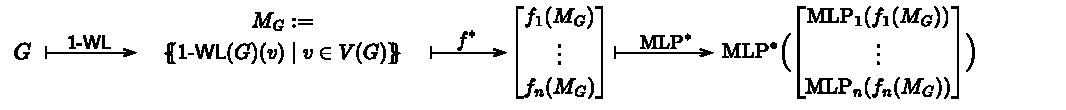
\includegraphics[width=\textwidth]{Figures/proof_sketch_wlnn_composition.pdf}
        \caption{The proof idea for \autoref{lem:composition_lemma}, how the constructed functions $f^*$ and $\mlp^*$ will work on input $G \in \cX$. Here we denote with $M_G$ the multiset of colors of the nodes of $G$ after applying the $\wl$ algorithm.}
        \label{fig:proof_idea_parallelism}
    \end{figure}
\end{proof}
    

\begin{lemma}\label[lemma]{lem:encoding-indicator-func1}
    Let $\cC$ be a collection of functions from $\cX$ to $\Rb$ computable by $\wlnn$ that is \wldisc. Then for all $G^* \in \cX$, there exists a function $h_{G^*}$ from $\cX$ to $\Rb$ computable by $\wlnn$, such that for all $G \in \cX: h_{G^*}(G) = 0$, if and only if, $G \wliso G^*$.
\end{lemma}

\begin{proof}
    Assume the above. For any $G_1, G_2 \in \cX$ with $G_1 \not\wliso G_2$, let $h_{G_1, G_2} \in \cC$ be the function distinguishing them, with $h_{G_1, G_2}(G_1) \neq h_{G_1, G_2}(G_2)$. We define the function $\overline{h}_{G_1,G_2}$ working over $\cX$ as follows:
    \begin{align}\label{eq:lemma_inidcator_function_1}
        \overline{h}_{G_1, G_2}(\cdot) &= |h_{G_1, G_2}(\cdot) - h_{G_1, G_2}(G_1)| \nonumber\\
        &= \max(h_{G_1, G_2}(\cdot) - h_{G_1, G_2}(G_1), \ 0) + \max(h_{G_1, G_2}(G_1) - h_{G_1, G_2}(\cdot), \ 0) \nonumber\\
        &= \text{ReLU}(h_{G_1, G_2}(\cdot) - h_{G_1, G_2}(G_1)) + \text{ReLU}(h_{G_1, G_2}(G_1) - h_{G_1, G_2}(\cdot))
    \end{align}
    Note, that in the equations above ``$h_{G_1, G_2}(G_1)$'' is a fixed constant and the resulting function $\overline{h}_{G_1, G_2}$ is non-negative.
    Let $G_1 \in \cX$ now be fixed, we will construct the function $h_{G_1}$ with the desired properties as follows:
    \begin{align}\label{eq:lemma_inidcator_function_2}
        h_{G_1}(\cdot) = \sum_{G_2 \in \cX, \ G_1 \not\wliso G_2} \overline{h}_{G_1, G_2}(\cdot).
    \end{align}
    Since $\cX$ is finite, the sum is finite and therefore well-defined. Next, we will prove that for a fixed graph $G_1 \in \cX$, the function $h_{G_1}$ is correct on input $G \in \cX$:
    \begin{enumerate}
        \item If $G_1 \wliso G$, then for every function $\overline{h}_{G_1, G_2}$ of the sum with $G_1 \not\wliso G_2$, we know, using \autoref{lem:wl_relation_equivalence}, that $\overline{h}_{G_1, G_2}(G)$ is equal to $\overline{h}_{G_1, G_2}(G_1)$ which is by definition $0$, such that $h_{G_1}(G) = 0$.
        \item If $G_1 \not\wliso G$, then $\overline{h}_{G_1, G}(G)$ is a summand of the overall sum, and since $\overline{h}_{G_1, G}(G) > 0$, 
        we can conclude $h_{G_1}(G) > 0$ due to the non-negativity of each function $\overline{h}_{G_1, G_2}$.
    \end{enumerate}
    Using \cref{lem:composition_lemma}, we can conclude that for any $G \in \cX$, $h_G$ is computable by $\wlnn$, as we can encode \autoref{eq:lemma_inidcator_function_2} via a multilayer perceptron where the factor ``$h_{G_1, G_2}(G_1)$'' of \autoref{eq:lemma_inidcator_function_1} is just a constant.
\end{proof}

\begin{lemma}\label[lemma]{lem:encoding-indicator-func2}
    Let $\cC$ be a collection of functions from $\cX$ to $\Rb$ computable by $\wlnn$ so that for all $G^* \in \cX$, there exists $h_{G^*} \in \cC$ satisfying $h_{G^*}(G) = 0 $ if and only if $G \wliso G^*$ for all $G \in \cX$. Then for every $G^* \in \cX$, there exists a function $\varphi_{G^*} $ computable by $\wlnn$ such that for all $G \in \cX$: $\varphi_{G^*}(G) = \mathds{1}_{G \wliso G^*}$.
\end{lemma}
\begin{proof}
    Assuming the above. Due to $\cX$ being finite, we can define for every graph $G^*$ the constant:
    \begin{equation*}
        \delta_{G^*} \coloneqq \frac{1}{2} \min_{G \in \cX , \  G \not\wliso G^*} |h_{G^*}(G)| > 0.
    \end{equation*}
    With this constant, we can use a so-called ``bump'' function working from $\Rb$ to $\Rb$ that is similar to the indicator function. We define this function for parameter $a \in \Rb$ with $a > 0$ as:
    \begin{align}\label{eq:lemma_encoding_indicator_func2}
        \psi_a(x) &\coloneqq \max(\frac{x}{a} -1,\ 0) + \max(\frac{x}{a}+1, \ 0) - 2 \cdot \max(\frac{x}{a}, \ 0) \nonumber\\
        &= \text{ReLU}(\frac{x}{a} -1) + \text{ReLU}(\frac{x}{a}+1) - 2 \cdot \text{ReLU}(\frac{x}{a})
    \end{align}
    The interesting property of $\psi_a$ is that it maps every value $x$ to $0$, except when $x$ is being drawn from the interval $(-a, a)$. In particular, it maps $x$ to $1$ if and only if $x$ is equal to $0$. See \autoref{fig:bump_function} for a plot of the relevant part of this function with exemplary values for $a$.
    
    We use these properties to define for every graph ${G^*} \in \cX$ the function $\varphi_{G^*}(\cdot) \coloneqq \psi_{\delta_{G^*}} (h_{G^*}(\cdot))$. 
    We will quickly demonstrate that this function is equal to the indicator function, for this let $G^*$ be fixed and $G$, an arbitrary graph from $\cX$, the input:
    \begin{enumerate}
        \item If $G \wliso G^*$, then $h_{G^*}(G) = 0$ resulting in $\varphi_{G^*}(G) = \psi_{\delta_{G^*}}(0) = 1$.
        \item If $G \not\wliso G^*$ then $h_{G^*}(G) \neq 0$, such that $|h_{G^*}(G)|> \delta_{G^*}$ so that $h_{G^*}(G) \not\in (-\delta_{G^*}, \delta_{G^*}) $ resulting in $\varphi_{G^*}(G) = 0$.
    \end{enumerate}
    Note that we can encode $\varphi_{G^*}$ using \autoref{eq:lemma_encoding_indicator_func2} via a multilayer perceptron, where $\delta_{G^*}$ is a constant. With \autoref{lem:composition_lemma} we can therefore conclude that $\varphi_{G^*}$ is computable by $\wlnn$ for every graph ${G^*} \in \cX$.
\end{proof}

\begin{figure}[H]
    \centering
    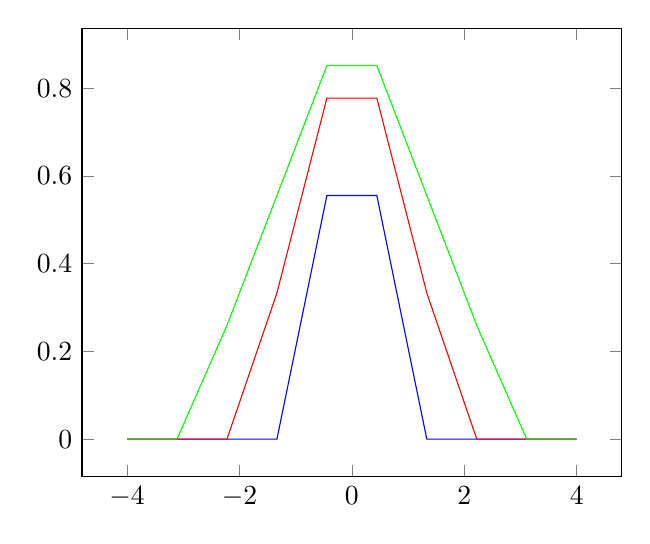
\begin{tikzpicture}
    \begin{axis}
    \addplot[domain=-4:4, samples=10, color=blue,]{max(x-1,0) + max(x+1,0) - 2*max(x,0)};
    \addplot[domain=-4:4, samples=10, color=red,]{max(x/2-1,0) + max(x/2+1,0) - 2*max(x/2,0)};
    \addplot[domain=-4:4, samples=10, color=green,]{max(x/3-1,0) + max(x/3+1,0) - 2*max(x/3,0)};
    \end{axis}
\end{tikzpicture}
    \caption{Illustration of the so-called ``bump'' function $\psi_a(x)$ used in the proof of \cref{lem:encoding-indicator-func2} with different exemplary values for $a$.}
    \label{fig:bump_function}
\end{figure}

\begin{lemma}\label{lem:decompose_gnn_as_wl}
    Let $\mathcal{C}$ be a collection of functions from $\cX$ to $\Rb$ computable by $\wlnn$ such that for all $G^* \in \cX$, there exists $\varphi_{G^*} \in \cC$ satisfying $\forall G \in \cX: \varphi_{G^*}(G) = \mathds{1}_{G \wliso G^*}$. Then every function computable by a \gnn is also computable by $\wlnn$.
\end{lemma}

\begin{proof}
    Assume the above. For any function $\mathcal{A}$ computed by a \gnn that works over $\cX$ to $\Rb$, we show that it can be decomposed as follows for any $G \in \cX$ as input:
    \begin{align}\label{eq:gnn_decomposition}
        \mathcal{A}(G) &= \Bigl( \ \frac{1}{|\cX/\!{\wliso}(G)|}\sum_{G^* \in \cX} \mathds{1}_{G \wliso G^*} \Bigr) \cdot \mathcal{A}(G) \nonumber \\
        &= \frac{1}{|\cX/\!{\wliso}(G)|}\sum_{G^* \in \cX} \mathcal{A}(G^*) \cdot \mathds{1}_{G \wliso G^*} \nonumber \\
        &= \sum_{G^* \in \cX} \frac{\mathcal{A}(G^*)}{|\cX/\!{\wliso}(G^*)|}  \cdot \varphi_{G^*}(G)
    \end{align}
    where we denote with $\cX/\!{\wliso}(G^*)$ the set of all graphs $G$ over $\cX$ that are equivalent to $G^*$ according to the $\wliso$ relation.

    Since $\cA$ is permutation-invariant and \gnns are, at most, as good as the \wl algorithm in distinguishing non-isomorphic graphs, we can use the fact that for every pair of graphs $G, H \in \cX$ with $G \wliso H$: $\cA(G) = \cA(H)$. Therefore, we can decompose $\cA$ as indicated in \autoref{eq:gnn_decomposition} and encode it using a multilayer perceptron where $\frac{\cA(G^*)}{|\cX/\!{\wliso}(G^*)|}$ is a constant, and $\varphi_{G^*} \in \cC$ encodes the indicator function. Combined with the \autoref{lem:composition_lemma}, we can conclude that $\cA$ is computable by $\wlnn$. Important to note, we can only do this since $\cX$ is finite, making the overall sum finite and the cardinality of $\cX/\!{\wliso}(G^*)$ well-defined for all graphs.
\end{proof}

\subsection{Proof of \autoref{theorem:gnn_in_1wl}}
In this section we will prove the converse direction. We start with \cref{lem:1wl_color_upper_bound}, where we introduce an upper bound that we will use in \cref{lem:gnn_1wl_disc} to show that there exists a collection of \gnn-computable functions that is \wldisc. After that, we will prove a composition lemma with \cref{lem:composition_lemma_gnn} which is similar to the one we introduced in the previous section. From this point on, the proof continues as in the previous section and concludes the property to be proved in \cref{lem:decompose_wl_as_gnn}.

\begin{lemma}\label{lem:1wl_color_upper_bound}
    Let $G$ be an arbitrary graph with $n \coloneqq |V(G)|$ the number of nodes and $C: V(G) \rightarrow \Nb$ an arbitrary coloring of the graph $G$. Then the total number of possible tuples of the form:
    \begin{equation*}
        (C(v), \ \MSopen C(u) \mid u \in \cN(v) \MSclose),
    \end{equation*}
    for all $v \in V(G)$ can be upper bounded by:
    \begin{equation*}
        n \cdot \sum_{i=0}^{n-1} \binom{n+i -1}{i}.
    \end{equation*}
\end{lemma}

\begin{proof}
    Assume the above. For the first entry of the tuple, at most $n$ different colors exist since there are $n$ nodes. For the second entry, each node $v \in V(G)$ can have between $0$ and $n-1$ neighbors, such that the total number of possibilities is the sum over each cardinality of a multiset with $n$ different colors. In the end, we soundly combine both results by multiplying both together.
\end{proof}


\begin{lemma}[GNN \wldisc]\label{lem:gnn_1wl_disc}
    There exists a collection $\cC$ of functions from $\cX$ to $\Rb$ computable by \gnns that is \wldisc. Meaning for every $G_1, G_2 \in \cX$ with $G_1 \not\wliso G_2$ there exists $\cA \in C$ such that $\cA(G_1) \neq \cA(G_2)$.
\end{lemma}

\begin{proof}
Since $\cX$ is finite, we define $n \coloneqq \max \{ |V(G)| \mid G \in \cX \}$ to be the maximum number of nodes of a graph in $\cX$, and $k \coloneqq \max \{ l_G(v) \mid v \in V(G), G \in \cX \}$ to be the largest label of any node of a graph in $\cX$. Using \cref{lem:1wl_color_upper_bound}, we can compute an upper bound $m$ using $n$ for the number of distinct tuples. Note that, this bound holds true for all graphs in $\cX$. We will now construct a \gnn with $n$ layers working on input $G$ as follows:
\begin{align*}
    f^{(0)}(v) &\coloneqq l_G(v), \ \text{and}\\
    f^{(t)}(v) &\coloneqq \textsc{RELABEL}_{m,t}(f^{(t-1)}(v), \ \MSopen f^{(t-1)}(u) \mid u \in \cN(v)\MSclose), \quad 0 < t < n.
\end{align*}
Here $\textsc{RELABEL}_{m,t}$ is a function that maps the tuples injectively to an integer of the set:
\begin{align*}\{i \in \Nb \mid k + (t-1)\cdot m +1 \leq i \leq k + t \cdot m\}.
\end{align*}
This function exists as by the soundness of the upper bound of \cref{lem:1wl_color_upper_bound}, the cardinality of its co-domain is greater or equal than the one of its domain. Thereby, and with the injectiveness of $\textsc{RELABEL}_{m,t}$, we ensure that each \gnn layer maps a tuple to a new, previously unused color. Therefore, every layer of this \gnn computes a single iteration of the $\wl$ algorithm. Further, since the $\wl$ algorithm converges after at most $|V(G)| \leq n$ iterations, we set the number of layers to $n$. We ensure that the coloring computed by this \gnn after $n$ layers when applied on any graph $G \in \cX$ is similarly expressive as the coloring computed by the $\wl$ algorithm when applied on $G$.

We define the collection $C$ of functions computable by \gnns that is \wldisc as: 
\begin{align*}
    C \coloneqq \{ \cA: \cX \rightarrow \Rb, \ G \mapsto \textsf{Readout}_c(\MSopen f^{(n)}(v) \mid v \in V(G) \MSclose) \mid c \in \Nb \},
\end{align*}
where $\textsf{Readout}_c$ is the \textsf{Readout} function that returns the number of nodes colored as $c$ in the coloring of $f^{(n)}$.
\end{proof}

Similar to the proof in the previous section, we will use \cref{lem:composition_lemma_gnn} to introduce the ability to construct \gnns that take in as input multiple \gnns and then apply a multilayer perceptron to the combined output.

\begin{lemma}[Composition \gnn]\label{lem:composition_lemma_gnn}
    Let $C$ be a collection of function computable by \gnns. Further, let  $\cA_1, \dots , \cA_n \in C$ and $\mlp^\bullet$ a suitable multilayer perceptron, then \\$\hat{\cA}(\cdot) \coloneqq \mlp(\cA_1(\cdot), \dots, \cA_n(\cdot))$ is also computable by a \gnn.
\end{lemma}

\begin{proof}
    Further, for any $x \in \Rb^d$, we will use the notation $x[i]$ to indicate the $i$.th element of the vector $x$. Additionally, we indicate the merge and aggregation function used in layer $t$ by $\cA_i$ as $f^{(t)}_{\text{merge}, i}$ and $f^{(t)}_{\text{agg}, i}$. Similarly, does $\textsf{Readout}_i$ indicate the \textsf{Readout} function and $f^{(0)}_i$ the input function of $\cA_i$.
    
    We will prove the lemma by constructing $\hat{\cA}$. Let $T$ be the maximum number of layers of all $\cA_1, \dots, \cA_n$. We construct the \gnn $\hat{\cA}$ with $T$ layers, with the input layer working as follows on an input graph $G$:
    \begin{align*}
        \forall v \in V(G): \ \hat{f}^{(0)}(v) \coloneqq \begin{bmatrix}
            f^{(0)}_1(v)\\
            \vdots\\
            f^{(0)}_n(v)
        \end{bmatrix},
    \end{align*}
    and each other layer $0 < t \leq K$ uses the merge $\hat{f}^{(t)}_{\text{merge}}$ and aggregation $\hat{f}^{(t)}_{\text{agg}}$ functions as defined below:
    \begin{align*}
        \hat{f}^{(t)}_{\text{merge}} (\hat{f}^{(t-1)}(v), \ Agg) &:= \begin{bmatrix}
            f^{(t)}_{\text{merge}, 1}(\hat{f}^{(t-1)}(v)[1],\ Agg[1])\\
            \vdots\\
            f^{(t)}_{\text{merge}, n}(\hat{f}^{(t-1)}(v)[n],\ Agg[n])
        \end{bmatrix},\quad \text{and}\\
        \hat{f}^{(t)}_{\text{agg}}(\MSopen \hat{f}^{(t-1)}(w) \mid w \in \mathcal{N}(v) \MSclose ) &:= \begin{bmatrix}
            f^{(t)}_{\text{agg}, 1}(\MSopen f^{(t-1)}(w)[1] \mid w \in \mathcal{N}(v) \MSclose)\\
            \vdots\\
            f^{(t)}_{\text{agg}, n}(\MSopen f^{(t-1)}(w)[n] \mid w \in \mathcal{N}(v) \MSclose)
        \end{bmatrix}.
    \end{align*}
    Note that, not all $\cA_i$ will be comprised of $K$ layers. For these cases we define the missing functions as follows:
    \begin{align*}
        f^{(t)}_{\text{merge}, i}(\hat{f}^{(t-1)}(v), \ Agg) &\coloneqq \hat{f}^{(t-1)}(v), \quad \text{and}\\
        f^{(t)}_{\text{agg}, i}(\MSopen f^{(t-1)}(w) \mid w \in \mathcal{N}(v) \MSclose) &\coloneqq 0.
    \end{align*}
    These functions do not change anything, and only forward the result of the actual computation of $\cA_i$ to the last layer. Finally, we construct the \textsf{Readout} function of $\hat{\cA}$ as follows:
    \begin{align*}
        \textsf{Readout}(\MSopen \hat{f}^{(T)}(v) \mid v \in V(G) \MSclose) \coloneqq \mlp \circ \begin{bmatrix}
            \textsf{Readout}_1(\MSopen \hat{f}^{(T)}(v)[1] \mid v \in V(G) \MSclose)\\
            \vdots\\
            \textsf{Readout}_n(\MSopen \hat{f}^{(T)}(v)[n] \mid v \in V(G) \MSclose)
        \end{bmatrix}.
    \end{align*}
\end{proof}

As a consequence of the previous two lemmas, we find ourselves in a similar position as at the beginning of the proof in \cref{sec:proof_theorem:1wl_in_gnn}. Specifically, we have established, through \cref{lem:gnn_1wl_disc}, the existence of a collection $C$ of functions that can be computed by \gnns and can effectively distinguish any pair of graphs that are also distinguishable by the \wl algorithm. Furthermore, with \cref{lem:composition_lemma_gnn}, we have demonstrated that the composition of multiple \gnns and a multilayer perceptron remains computable by a single \gnn. Consequently, we can also apply the findings of \cref{lem:encoding-indicator-func1,lem:encoding-indicator-func2} to \gnns. Thus, we can conclude that for any fixed $G^* \in \cX$, the indicator function $\varphi_{G^*}$ working over $\cX$ with:
\begin{align*}
        \forall G \in \cX: \quad \varphi_{G^*}(G) := 
        \begin{cases}
            1, \quad \text{if $G \wliso G^*$}\\
            0, \quad \text{else}
        \end{cases},
\end{align*}
is computable by a \gnn.

\begin{lemma}\label{lem:decompose_wl_as_gnn}
    Let $\mathcal{C}$ be a collection of functions from $\cX$ to $\Rb$ computable by \gnns so that for all $G^* \in \cX$, there exists 
    $\varphi_{G^*} \in \cC$ satisfying $\forall G \in \cX: \varphi_{G^*}(G) = \mathds{1}_{G \wliso G^*}$. Then every function computable by $\wlnn$ is also computable by a \gnn.
\end{lemma}

\begin{proof}
    Assume the above. For any function $\cB$ computed by $\wlnn$ that works over $\cX$ to $\Rb$, we show that it can be decomposed as follows for any $G \in \cX$ as input:
    \begin{align}\label{eq:1wl_decomposition}
        \cB(G) &= \Bigl( \ \frac{1}{|\cX/\!{\wliso}(G)|}\sum_{G^* \in \cX} \mathds{1}_{G \wliso G^*} \Bigr) \cdot \cB(G) \nonumber \\
        &= \frac{1}{|\cX/\!{\wliso}(G)|}\sum_{G^* \in \cX} \cB(G^*) \cdot \mathds{1}_{G \wliso G^*} \nonumber \\
        &= \sum_{G^* \in \cX} \frac{\cB(G^*)}{|\cX/\!{\wliso}(G^*)|}  \cdot \varphi_{G^*}(G)
    \end{align}
    where we denote with $\cX/\!{\wliso}(G^*)$ the set of all graphs $G$ over $\cX$ that are equivalent to $G^*$ according to the $\wliso$ relation. Further, with \cref{lem:wl_relation_equivalence} we know that for any $G_1, G_2 \in \cX$ with $G_1 \wliso G_2: \cB(G_1) = \cB(G_2)$.
    
    We can encode $\cB$ as stated in \autoref{eq:1wl_decomposition} via a multilayer perceptron with $\frac{\cB(G^*)}{|\cX/\!{\wliso}(G^*)|}$ being constants and $\varphi_{G^*} \in \cC$ encoding the indicator function. Combined with the \autoref{lem:composition_lemma_gnn}, we can conclude that $\cB$ is computable by $\wlnn$. Important to note, we can only do this since $\cX$ is finite, making the overall sum finite and the cardinality of $\cX/\!{\wliso}(G^*)$ well-defined for all graphs.
\end{proof}